\providecommand{\curso}{Séptimo Básico}
\providecommand{\colegio}{Colegio Divina Pastora}
\providecommand{\tituloDocumento}{Evaluación grupal}
\providecommand{\subtituloDocumento}{La geometría del círculo}
\documentclass{DivinaPastora}

\begin{document}
%
\begin{tcenter}%
    \begin{tikzpicture}[ampersand replacement=\&,]%
        \matrix [matrix of nodes]% 
        {\noindent\Caja[Integrante n° 1][.6\linewidth][30pt] \&
        \noindent\Caja[Puntaje][.19\linewidth][30pt] \\
        \noindent\Caja[Integrante n° 2][.6\linewidth][30pt] \&
        \noindent\Caja[Nota][0.19\linewidth][30pt] \\};
    \end{tikzpicture}%
\end{tcenter}%

\titulo{Objetivos de la evaluación}
\begin{itemize}[nosep]
    \item Describir las relaciones entre el radio del círculo con el perímetro y área de este.
    \item Aplicar aproximaciones del perímetro y del área en la resolución de problemas contextualizados.
    \item Explicar y fundamentar:
    \begin{itemize}[label=\textbullet]
        \item Soluciones propias y los procedimientos utilizados.
        \item Resultados mediante definiciones, axiomas, propiedades y teoremas.
    \end{itemize}
\end{itemize}

\titulo{Instrucciones generales}
La evaluación es de trabajo colaborativo y con nota al libro.
En su desarrollo pueden usar calculadora, pero, es importante
que incluyan en sus respuestas tanto los cálculos como procedimientos
necesarios para responder el enunciado.

\titulo{Pauta de cotejo}
En la corrección de la evaluación, se le asignará puntaje a cada respuesta según
los criterios que se encuentran detallados en la tabla a continuación.\par
\begin{tblr}{width=\linewidth,colspec={X[1,c]|X[6]}, hline{1,Z} = {1}{-}{}, hline{1,Z} = {2}{-}{}, 
    hlines, cells={valign=m}, row{2,4} = {bg=black!15}}
    Puntaje asignado & \SetCell{c} Criterios o indicadores \\
    \SetCell[c=2]{c} {\bfseries\sffamily Parte 1:} Explicar definiciones y propiedades \\
    $100$\% & La respuesta describe el concepto de manera clara y haciendo referencia 
    de carac\-terís\-ticas claves. Respuestas incompletas tienen puntaje intermedio. \\
    \SetCell[c=2]{c} {\bfseries\sffamily Parte 2:} Resolución de problemáticas \\
    +40\% & Señala clara y correctamente cuál es la solución o el resultado de la pregunta hecha
    en el enunciado. \\ 
    +60\% & Incluye un desarrollo que relata de manera clara y ordenada los procedimientos 
     \mbox{necesarios} para solucionar la problemática. En caso de estar incompleto o con 
     \mbox{errores} el desarrollo, se asignará puntaje parcial si se muestra dominio de los 
     con\-tenidos y conceptos involucrados. \\
    0\% &  La respuesta es incorrecta. De haber desarrollo, este tiene errores conceptuales.\\
\end{tblr}    

\begin{center}
\begin{tikzpicture}[ampersand replacement=\&,]
    %\node (A) [opacity=0.4] {\includegraphics[width=2cm]{../flork3.jpg}};
    \node (B) [font=\slshape,text width=12cm]
    {``Cree en ti mismo y en lo que eres. Sé consciente de que hay algo en tu interior %
    que es más grande que cualquier obstáculo''};
    \node [left=0mm of B,opacity=0.4] {\pgfornament[width=2cm]{37}};
    \node [right=0mm of B,opacity=0.4] {\pgfornament[width=2cm]{38}};
\end{tikzpicture}
\end{center}

\parte Define y explica los conceptos que se encuentran a continuación. 
Para esto, considera que la persona revisando las respuestas no maneja los 
conceptos involucrados, es decir, usted se los debe enseñar.
%
%\begin{tikzpicture}[overlay]
%    \fill [yshift=-5mm,xshift=-5mm] (current page.north east) circle (3mm);
%\end{tikzpicture}
%
\pregunta ¿Qué es una circunferencia?  
¿Es la figura que se encuentra a continuación una circunferencia? ¿Sí? ¿No? ¿Por qué? 
%% todos los puntos se encuentran a la misma distancia del centro
%% hace referencia a sus partes: tiene centro y un lado
\begin{center}
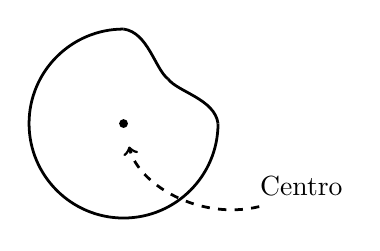
\begin{tikzpicture}[ampersand replacement=\&,scale=0.4,line width=1pt]
    \draw (3,0) .. controls (15:3) and (30:2) .. (45:2);
    \draw (45:2) .. controls (60:2) and (75:3) .. (0,3); 
    \draw (0,3) arc [start angle=90, end angle=360, radius=3];
    \fill (0,0) circle (4pt);
    \node (A) at (4,-2) [anchor=west] {Centro};
    \draw [->,dashed,shorten >=3mm] (A) to [bend left=45] (0,0);
\end{tikzpicture}
\end{center}
\respuesta[5]

\pregunta ¿Qué representa el perímetro de un círculo? ¿Cómo se puede estimar 
el perímetro de un círculo?
%% el largo de la cuerda que forma el circulo 
%% p = 2*pi*r  o bien p = d*pi
\respuesta[5]

\pregunta ¿Qué representa el área del un círculo? ¿Cómo se puede estimar el 
área de un círculo?  %% es el espacio que ocupa, la cantidad de papel
%% a = pi*r^2
\respuesta[5]

\parte Use el material facilitado por el profesor para responder los problemas 
que se encuentran a continuación. Cada una de sus respuestas debe estar 
fundamentada por un desarrollo, que incluya los cálculos y procedimientos necesarios 
para solucionar la problemática.
%
%\begin{center}
%    \includegraphics[width=.4\linewidth,trim=0.5cm 0.5cm 0.4cm 0.4cm,clip]{~/Downloads/cdrom.pdf}
%\end{center}

\pregunta ¿Cuál es el área de la superficie del CD?
\desarrollo[5]
\respuesta[2]
\pregunta Si el tamaño del CD aumenta en 200 veces, ¿Cuántas personas 
podrían sentarse alrededor de este CD gigante?
\desarrollo[7]
\respuesta[5]

\pregunta ¿Cuántas personas se podrían 
colocar en la superficie del CD gigante?
\desarrollo[7]
\respuesta[5]

\vspace{3cm}\hspace{11cm}\tikz[]{\node [rotate=-30,opacity=0.4  ]{\pgfornament[width=4cm]{122}};}

\tikz[remember picture,overlay] {%
    \foreach \x in {0,1,...,15} {
        \draw [line width=1pt] 
            ($(current page.south west) + (\x +1,0)$) -- +(0,2) node[pos=1,above] {$\x$};
    }
    \foreach \xx in {0,0.1,...,15} {
        \draw []
            ($(current page.south west) + (\xx +1,0)$) -- +(0,1);
    }
}

\end{document}